% !TEX program = xelatex

% Základní balíčky
\documentclass[10pt,a4paper]{article}
\usepackage[utf8]{inputenc}
\usepackage[T1]{fontenc}
\usepackage{graphicx}
\usepackage{wrapfig}
\usepackage{nonfloat}
\usepackage{amsmath}
\usepackage{amssymb}
\usepackage{mathtools}
\usepackage{hyperref}
\usepackage{gensymb}
\usepackage{listings}
\usepackage[top = 1cm, bottom = 1cm, left = 1cm, right = 1cm]{geometry}

% Language-related
\usepackage[czech]{babel}
\AtBeginDocument{\shorthandoff{-}}
\usepackage{csquotes}
\usepackage{polyglossia}
\setmainlanguage{czech}
\setotherlanguage{greek}

% Bibtex je oficiálně mrtka
% \usepackage[backend=bibtex,style=verbose-trad2]{biblatex}
% \usepackage{etoolbox}
% \patchcmd{\thebibliography}{\section*{\refname}}{}{}{}
% \bibliography{protokol}

% Pro titulní stránku
\usepackage{titlesec}
\usepackage{setspace}
\usepackage{framed}
\usepackage{array}

% Vlastní balíčky
\usepackage{gnuplottex}
\usepackage{epstopdf}
\usepackage{csvsimple}
\usepackage{units}
\usepackage{subfig}
\usepackage{pdfpages}
\usepackage{multirow}

\usepackage{soul}

\usepackage{calc}
\newcommand*{\mask}[2]{\mathord{\makebox[\widthof{\(#1\)}]{\(#2\)}}}




\renewcommand{\U}[1]{\ensuremath{\,\mathrm{#1}}}
\newcommand{\°}{\degree}

\newcommand{\titjmeno}{Michal Grňo}
\newcommand{\titobor}{FOF}


\newcommand{\titcislo}{A17}
\newcommand{\titnazev}{Zeemanův jev}
\newcommand{\titmereni}{19. 11. 2020}
\newcommand{\titodevzdani}{4. 12. 2020}


\renewcommand{\t}[1]{\mathrm{#1}}


\begin{document}


\thispagestyle{empty}
\newgeometry{top = 2.5cm, bottom = 0cm, left = 2.5cm, right = 3cm}

{%T tomto je uzavřena celá titulka
%Tloušťka rámečku
\setlength{\fboxrule}{1.5pt}

\noindent
\framebox{
\begin{minipage}{\textwidth}
\setlength{\parindent}{17.62482 pt}
\phantom{d}

\begin{minipage}{0.6\textwidth}
{
\Large Kabinet výuky obecné fyziky, UK MFF\\
}
\vspace*{0.2cm}

{
\bfseries
\huge Fyzikální praktikum %ČÍSLO
}
\end{minipage}
\begin{minipage}{0.4\textwidth}
\begin{center}
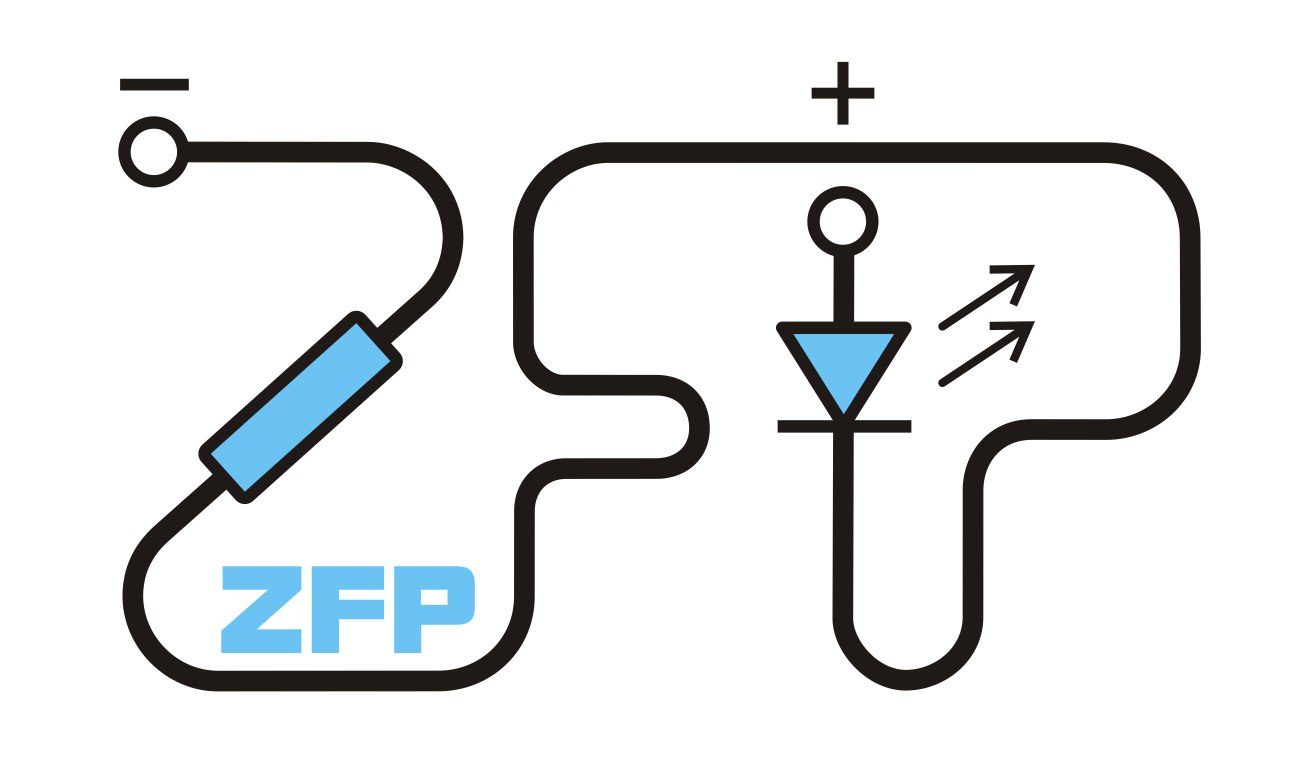
\includegraphics[width=4.5cm]{ZFP.jpg}
\end{center}
\end{minipage}\\\\

%\vspace*{0.5cm}

{
\setstretch{1.5}
\Large
\noindent
Úloha č. \titcislo

\noindent
Název úlohy: \titnazev

\noindent
Jméno: \titjmeno
\hspace*{\fill}
Obor: \titobor

\noindent
Datum měření: \titmereni
\hspace*{\fill}
Datum odevzdání: \titodevzdani

\phantom{d}
}
\end{minipage}
}
%Konec horního rámečku

{
\phantom{d}

\Large
Připomínky opravujícího:\\
\vspace*{6.75cm}
}

\newcommand{\linka}{\noalign{\hrule height 1pt}}
\newcommand{\linkadva}{\noalign{\hrule height 1.5pt}}
\setlength\extrarowheight{9.5pt}
\Large
\noindent
\begin{tabular}{!{\vrule width 1.5pt} l !{\vrule width 1pt} c !{\vrule width 1pt} c !{\vrule width 1.5pt}}
\linkadva
   & Možný počet bodů & Udělený počet bodů \\\linkadva
  Práce při měření & 0-3 &  \\\linka
  Teoretická část & 0-2 &  \\\linka
  Výsledky a zpracování měření & 0-9 &  \\\linka
  Diskuse výsledků & 0-4 &  \\\linka
  Závěr & 0-1 &  \\\linka
  Použitá literatura & 0-1 &  \\\linkadva
  \hspace*{\fill} \textbf{Celkem} \hspace*{\fill}& max. 20 &  \\
\linkadva
\end{tabular}
\phantom{d}

Posuzoval: \hspace*{\fill}dne:~~~~~~~~~~~~~~~~~

}%Konec uzavření titulky
\newpage
\newgeometry{top = 2cm, bottom = 2cm, left = 2cm, right = 2cm}
\setcounter{page}{1}
\setmainfont{Linux Libertine O}




\section{Pracovní úkoly}
\begin{enumerate}

    \item Proměřte závislost magnetické indukce na proudu magnetu.
    \item Pomocí kamery změřte ve směru kolmém k magnetickému poli rozštěpení červené spektrální čáry kadmia pro 8-10 hodnot magnetické indukce. Snímky vyhodnoťte vhodným programem podle návodu. Určete polarizaci složek rozštěpené čáry.
    \item \st{Totéž proveďte pro 6-8 hodnot indukce při pozorování ve směru magnetického pole. Opět určete polarizaci.}
    \item \st{Výsledky obou sérií měření vzájemně porovnejte.} Určete chyby měření.
    \item Kvalitativně popište výsledky pozorování Zeemanova jevu \st{na zelené čáře kadmia ($\lambda = 508.6 \U{nm}$)}.
\end{enumerate}

\section{Teoretická část}
V práci budeme měřit štěpení spektrálních čar při normálním Zeemanově jevu. K tomu dochází, když se spektrální čára o vlnové délce $\lambda_0$ vlivem externího magnetického pole rozštěpí na tři čáry $\lambda_0 - \Delta\lambda, \; \lambda_0, \; \lambda_0 + \Delta\lambda$. Tyto nově vzniklé čáry čáry budeme značit písmeny $z, x, y$ (postupně od nejmenší vlnové délky po největší). Změna vlnové délky $\Delta\lambda$ je přímo úměrná síle magnetické indukce, platí pro ni vzorec
\begin{equation}
    \Delta\lambda = \frac{e}{m_{\mathrm{e}}} \, \frac{\lambda_0^2 B}{4 \pi c} \: ,
    \label{eq-merny-naboj}
\end{equation}
kde $e$ je elementární náboj, $m_{\mathrm{e}}$ hmotnost elektronu, $B$ magnetická indukce externího pole a $c$ rychlost světla. [1] My budeme pro měření používat červenou spektrální čáru kadmiové výbojky s $\lambda_0=643.8 \U{nm}$. Protože experiment vyžaduje velmi citlivý aparát, budeme pracovat se spektrometrem s Lummerovou-Gehrckeovou deskou. V difrakčním obrazci spektrometru typicky jedna vlnová délka $\lambda$ odpovídá několika interferenční maximům $\lambda_k$,  kde $k$ je přirozené číslo. Pro $k$-té interferenční maximum odpovídající čárám $z,x,y$ budeme používat značení
\begin{equation*}
    z_k, \; x_k, \; y_k \: .
\end{equation*}
Další význačná vlnová délka je tzv. \textit{velikost disperzní oblasti} $\Delta\lambda_{\mathrm{D}}$, která udává, jak jsou od sebe na stupnici spektrometru vzdálená interferenční maxima jednotlivých řádů – je-li tedy například $\Delta\lambda = \Delta\lambda_{\mathrm{D}}$, potom maximum $y_k$ splývá s maximem $x_{k+1}$. Velikost disperzní oblasti pro Lummerův-Gehrckeův spektrometr lze vypočítat jako
\begin{equation*}
    \Delta\lambda_{\mathrm{D}} = \frac{\lambda^2}{2d\sqrt{n^2-1}} \: ,
\end{equation*}
kde $d=4.04 \U{mm}$ je tloušťka desky, $\lambda\approx\lambda_0=643.8 \U{nm}$ je vlnová délka světla které používáme k difrakci (v našem případě červená čára Cd) a $n$ je index lomu destičky, v našem případě
\begin{equation*}
    n = 1.44263 + \frac{7.065}{\lambda/\!\U{nm} - 144}
    = 1.45677 \: . \; \text{ [1]}
\end{equation*}
Pro použitý aparát tedy máme
\begin{equation}
    \Delta\lambda_{\mathrm{D}} = 0.0484 \U{nm} \: .
    \label{eq-velikost-disp-obl}
\end{equation}
V difrakčním obrazu spektrometru ve skutečnosti neměříme přímo vlnovou délku, ale difrakční úhel, který budeme značit $\vartheta$. V nejjednodušší aproximaci platí $\vartheta \propto \lambda$. V takové aproximaci platí:
\begin{equation*}
    \Delta\lambda = \frac{\alpha}{\beta} \, \Delta\lambda_{\mathrm{D}} \: ,
\end{equation*}
kde $\alpha$ značí \textit{úhlový posun}, tj. rozdíl mezi úhlem $\vartheta$ čar $\lambda_0$ a $\lambda_0 + \Delta\lambda$, a $\beta$ značí \textit{úhlovou odlehlost} sousedních řádů. [1] Aproximace $\vartheta \propto \lambda$ však není úplně přesná, obzvlášť v okolí úhlu $\vartheta = 90\°$, kde budeme měřit. Lepší odhad nám dává kvadratická závislost
\begin{equation}
    \Delta\lambda =
    \Big( \big( \varrho + \varrho^{-1} \big) \, \xi + \big( \varrho - \varrho^{-1} \big) \, \xi^2 \Big)
    \, \Delta\lambda_{\mathrm{D}} \: ,
    \label{eq-kvadraticka}
\end{equation}
kde $\varrho$ a $\xi$ jsou proměnné, které lze odhadnout z poloh několika prvních interferenčních maxim:
\begin{equation*}
    \varrho = \frac{x_1 - x_0}{x_2 - x_1} \: , \quad
    \xi = \frac{y_1 - x_1}{x_2 - x_0} \: .
    \; \text{ [1]}
\end{equation*}
Tento odhad stále není ideální, protože ze všech identifikovaných peaků využijeme pouze $x_0, x_1, x_2$ a $y_1$, pro naše účely ale poskytuje dostatečnou přesnost.



\section{Měření a zpracování dat}
Nejprve jsme proměřili kalibrační křivku cívky. Protože se jedná o cívku s jádrem [2], očekáváme, že pro nízké proudy půjde o lineární závislost s větší směrnicí, která se následně „zlomí“ v bodě nasycení jádra. Naměřenou závislost (viz obrázek č.~\ref{img-kalibrace}) jsme proložili dvakrát lomenou čárou, jako parametry regrese jsme použili směrnice i body lomu. Výsledná závislost~je:
\begin{equation}
    b(x) = 0.0808 \, x - 0.030 \, (x-8.9) \, H(x-8.9) - 0.023 \, (x-11.1) \, H(x-11.1) \: ,
    \label{eq-magnetic-fit}
\end{equation}
kde $b$ je magnetická inducke v jednotkách $\U{T}$, $x$ je proud v jednotkách $\U{A}$ a $H(x)$ je Heavisidova schodová funkce. Odchylka naměřeného $B$ od fitu se pohybuje pod $6 \U{mT}$.

\begin{figure}[t]
    \centering
    \begin{gnuplot}[terminal=epslatex,terminaloptions={color size 15cm, 8cm}]
        load 'kalibrace.plt'
        set key top left
        set xlabel '$I \, [\U{A}]$'
        set ylabel '$B \, [\U{T}]$'
        set format y '%.1f'

        set y2tics
        set y2range [0:10]
        set y2label '$\Delta B \, [\U{mT}]$'

        plot 'data/kalibrace_magnetu_Hallova_sonda.dat' using 1:($2/10) t 'data $B(I)$' lc rgb 'black', B(x) t 'fit $B(I)$' lc rgb 'red', 'data/kalibrace_magnetu_Hallova_sonda.dat' using 1:(1000*abs($2/10 - B($1))) axes x1y2 pt 4 t 'chyba $\Delta B$'
    \end{gnuplot}
    \caption{Kalibrace závislosti magnetické indukce na proudu, proložená lomenou čárou.}
    \label{img-kalibrace}
\end{figure}


Následně jsme měřili difrakční obrazce pro proudy cívkou $5\U{A}$ až $14\U{A}$. Vypočítané odpovídající hodnoty magnetické inducke jsou v tabulce č. \ref{tab-proudy}, chyba $B$ v tabulce je vypočítaná pouze z chyby $I$ a směrnice grafu v daném místě, chyba fitu $B(I)$ není zohledněna.

\phantom{.}
\begin{minipage}{\linewidth}
    \centering
    \vspace{\baselineskip}
    \begin{tabular}{ rl|rl }
        \multicolumn{2}{c|}{$I [\U{A}]$} & \multicolumn{2}{c}{$B [\U{T}]$} \\\hline
        $5.00$ & $\!\pm\; 0.10$ & $0.404$ & $\!\pm\; 0.008$ \\
        $6.05$ & $\!\pm\; 0.10$ & $0.489$ & $\!\pm\; 0.008$ \\
        $7.00$ & $\!\pm\; 0.10$ & $0.566$ & $\!\pm\; 0.008$ \\
        $8.04$ & $\!\pm\; 0.10$ & $0.650$ & $\!\pm\; 0.008$ \\
        $10.06$ & $\!\pm\; 0.10$ & $0.778$ & $\!\pm\; 0.005$ \\
        $11.00$ & $\!\pm\; 0.10$ & $0.825$ & $\!\pm\; 0.005$ \\
        $12.00$ & $\!\pm\; 0.10$ & $0.856$ & $\!\pm\; 0.003$ \\
        $13.06$ & $\!\pm\; 0.10$ & $0.886$ & $\!\pm\; 0.003$ \\
        $14.16$ & $\!\pm\; 0.10$ & $0.917$ & $\!\pm\; 0.003$
    \end{tabular}
    \vspace{5pt}
    \tabcaption{Naměřené proudy a vypočítané magnetické indukce bodů, kde byl pořízen difrakční obrazec.}
    \label{tab-proudy}
    \vspace{\baselineskip}
\end{minipage}

Výstupem byla sada digitálních obrázků jako je obrázek č.~\ref{img-difrak-preview}, které zachytil CCD čip v aparátu spektrometru.
Pomocí programu Octave jsme z obrázků vybrali řez prostředkem obrázků, omezili se na červený kanál a do datových souborů exportovali průběh jasu a polohu maxim. Toho bylo dosaženo pomocí následujícího kódu:
\lstinputlisting[language=Octave]{./extract-image-data.m}
Automaticky označená maxima bylo ještě potřeba ručně promazat – program Octave jako maximum označil i skoky v jasu, které způsobila komprese obrázků. Tím jsme pro každý proud $I$ dostali sadu maxim $z_k, x_k, y_k$ jako jsme předpokládali v teorii. Příklady získaných dat jsou v obrázcích číslo \ref{img-rez-5A}, \ref{img-rez-9A} a \ref{img-rez-14A}.


\begin{figure}[p]
    \centering
    \vspace{1em}
    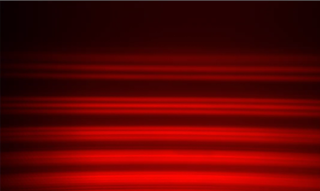
\includegraphics[width=8cm]{difrak-preview.png}
    \caption{Difrakční obrazec pro $I=5\U{A}$.}
    \label{img-difrak-preview}
\end{figure}

\begin{figure}[p]
    \centering
    \begin{gnuplot}[terminal=epslatex,terminaloptions={color size 17cm, 7cm}]
        file = '5A'
        load 'plotfile.plt'
    \end{gnuplot}
    \caption{Jas na řezu snímkem při $I=5\U{A}$.}
    \label{img-rez-5A}
\end{figure}

\begin{figure}[p]
    \centering
    \begin{gnuplot}[terminal=epslatex,terminaloptions={color size 17cm, 7cm}]
        file = '9A'
        load 'plotfile.plt'
    \end{gnuplot}
    \vspace{-2em}
    \caption{Jas na řezu snímkem při $I=9\U{A}$.}
    \label{img-rez-9A}
\end{figure}

\begin{figure}[p]
    \centering
    \begin{gnuplot}[terminal=epslatex,terminaloptions={color size 17cm, 7cm}]
        file = '14A'
        load 'plotfile.plt'
    \end{gnuplot}
    \caption{Jas na řezu snímkem při $I=14\U{A}$.}
    \label{img-rez-14A}
\end{figure}

\begin{figure}[p]
    \centering
    \begin{gnuplot}[terminal=epslatex,terminaloptions={color size 18cm, 7cm}]
        set xlabel '$I \, [\U{A}]$'
        set ylabel '$\vartheta \, [\U{px}]$'
        load 'all_peaks.plt'
    \end{gnuplot}
    \caption{Poloha naměřených peaků pro různé proudy. Hvězdička značí $z_k$, čtvereček $x_k$ a kolečko $y_k$. Barvy odlišují jednotlivá interferenční maxima.}
    \label{img-all-peaks}
\end{figure}

Dále bylo třeba z naměřených peaků určit $\Delta\lambda$ pro jednotlivé proudy $I$. Dosazením do rovnice \eqref{eq-kvadraticka} jsme dostali hodnoty $\Delta\lambda/\Delta\lambda_{\mathrm{D}}$, viz tabulka č. \ref{tab-lambdas}. Dále jsme pomocí \eqref{eq-velikost-disp-obl} a \eqref{eq-magnetic-fit} vyjádřili závislost $\Delta\lambda(B)$ a vynesli ji do grafu v obrázku č. \ref{img-lambda-vs-indukce}.
\begin{table}[h!]
    \centering
    \begin{tabular}{ r|c|c|c }
        $I \, [\!\U{A}]$ &
        $\rho$ & $\xi$ &
        $\Delta\lambda \, / \Delta\lambda_{\mathrm{D}}$
        \csvreader[ head to column names ]{zprac2/lambdas.csv}{}
        {
            \csviffirstrow{\\\hline}{\\}
            \proud & \koefRho & \koefXi & \posun
        }
    \end{tabular}
    \caption{Výpočet změny vlnové délky pro různé proudy.}
    \label{tab-lambdas}
\end{table}

\begin{figure}[p]
    \centering
    \begin{gnuplot}[terminal=epslatex,terminaloptions={color size 14cm, 6cm}]
        load 'kalibrace.plt'
        set datafile separator ','

        f(x) = a*x
        fit f(x) 'zprac2/lambdas.csv' using (B($1)):($4*0.0484*1000) via a

        set key top left
        set xlabel '$B\,[\!\U{T}]$'
        set ylabel '$\Delta\lambda \, [\!\U{pm}]$'
        set xrange [0.3:1]
        plot 'zprac2/lambdas.csv' using (B($1)):($4*0.0484*1000) t 'data', f(x) t 'fit'
    \end{gnuplot}
    \caption{Rekonstruovaná závislost délkového posunu na magnetické indukci.}
    \label{img-lambda-vs-indukce}
\end{figure}

\begin{wrapfigure}{R}{8cm}
    \centering
    \begin{gnuplot}[terminal=epslatex,terminaloptions={color size 7.5cm, 5cm}]
        unset xtics
        unset ytics
        set yrange [35:260]
        set key bottom right
        plot 'zprac1/9A a.png_raw.dat' w l lc rgb 'black' t 'pozice A', 'zprac1/9A b.png_raw.dat' w l lc rgb 'red' t 'pozice B'
    \end{gnuplot}
    \caption{Vliv orientace polarizačního filtru na pozorovaný difrakční obrazec.}
    \label{img-polarizace}
\end{wrapfigure}

\noindent Body v grafu na obr. č. \ref{img-lambda-vs-indukce} jsme proložili přímkou která prochází počátkem. Směrnice fitu je:
\begin{equation*}
    a = (19.22 \pm 0.16) \U{pm / T} \: .
\end{equation*}
Porovnáním s \eqref{eq-merny-naboj} potom dostáváme
\begin{equation*}
    \frac{e}{m_{\mathrm{e}}}
    = a \, \frac{4 \pi c}{\lambda_0^2}
    = (1.747 \pm 0.015) \cdot 10^{11} \U{C / kg} \: .
\end{equation*}

Nakonec jsme kvalitativně porovnali vliv orientace polarizačního filtru na pozorovaný difrakční obrazec. Nejrve jsme polarizační filtr umístili do polohy A, kde vymizely boční čáry $y, z$. Následně jsme filtr otočili o $90\°$ do polohy B. Pozorovali jsme, že v této poloze se boční čáry opět objevily, naopak zmizela čára $x$ (viz obrázek \ref{img-polarizace}). To indikuje, že čáry jsou lineárně polarizované, centrální čára kolmo k bočním čarám.

\pagebreak

\section{Diskuse}
Ze 106 identifikovaných peaků (viz obrázek č. \ref{img-all-peaks}) jsme jich pro výpočet $\Delta\lambda / \Delta\lambda_{\mathrm{D}}$ pomocí vzorce \eqref{eq-kvadraticka} použili pouze $4 \cdot 10 = 40$. Využitím všech peaků bychom jistě dosáhli přesnějšího výsledku, vyžadovalo by to ovšem sofistikovanější statistickou analýzu.

Fit v obrázku č. \ref{img-lambda-vs-indukce} jsme prováděli za předpokladu, že chyby všech bodů jsou stejné. Chybu $\Delta\lambda$ nedokážeme určit (protože je to hodnota získaná fitem funkce tří parametrů na tři body, viz \eqref{eq-kvadraticka}). Chybu $B$ lze usoudit z grafu v obrázku č. \ref{img-kalibrace} a z tabulky č. \ref{tab-proudy}; vidíme, že na celém intervalu máme chybu řádově v jednotkách $\U{mT}$. Předpoklad stejných chyb je tedy oprávněný.

Při měření jsme nepracovali s předehřátým elektromagnetem, ani jsme nečekali, až se jeho teplota ustálí. V průběhu měření se tedy jeho teplota vlivem protékajícího proudu výrazně měnila. Protože jsme ovšem používali zdroj konstantního proudu, na sílu magnetického pole neměla tato změna teploty vliv.

V obrázcích \ref{img-rez-9A} a \ref{img-rez-14A} je vidět, že maxima vyšších řádů zanikají v důvodu příliš vysoké expozice. Snížením jasu výbojky, snížením citlivosti CCD čipu nebo zvýšením clonového čísla bychom dosáhli ještě vyššího počtu identifikovaných peaků. Protože jsme ovšem v této práci maxima vysokých řádů nezapočítávali, neměla by tato volba na současný výsledek vliv.



\section{Závěr}
Podařilo se proměřit normální Zeemanův jev pro červenou čáru kadmia v magnetickém poli od $0.4 \U{T}$ do $0.9 \U{T}$. V difrakčních obrazcích se podařilo identifikovat 106 peaků, z nich 40 bylo použito k vypčítání závislosti změny vlnové délky $\Delta\lambda$ na magnetické indukci $B$. Z této závislosti se poté podařilo odhadnout měrný náboj elektronu
\begin{equation*}
    \frac{e}{m_{\mathrm{e}}}
    = (1.747 \pm 0.015) \cdot 10^{11} \U{C / kg} \: ,
\end{equation*}
což je v souladu s tabulkovou hodnotou. Podařilo se demonstrovat, že čáry $z,x,y$ jsou lineárně polarizované; $x$ je polarizované kolmo k $z,y$.

\section{Literatura}
[1] Praktikum částicové a jaderné fyziky. Zeemanův jev. 2002. \\ Dostupné z: \url{https://physics.mff.cuni.cz/vyuka/zfp/_media/zadani/texty/txt_417.pdf}.
\\[10pt]
[2] DANIŠ, Stanislav. Instrukce k absolvování distanční formy úlohy A-17 v rámci Praktika IV. 2020. \\ Dostupné z: \url{https://physics.mff.cuni.cz/vyuka/zfp/_media/zadani/texty/da_417.pdf}.

\end{document}
